
\section{Követelmények}

A mellékelt bináris 64 bites Windows operációs rendszerhez készült, azonban a forráskód a három legnagyobb asztali operációs rendszer (Windows, Linux, OS X) bármelyikére lefordítható, 32 és 64 bites változatban is, ennek menetéről bővebben a következő fejezet ad felvilágosítást.

Mivel a megjelenítő OpenGL alapú, ezért a futtató számítógépen elérhetőnek kell lennie az OpenGL 3.3-as verziójának. Ezt a verziót mind az integrált, mind a dedikált videokártyák évekre visszamenőleg támogatják. Ha nem vagyunk biztosak a támogatott verzióban, akkor a grafikus meghajtóprogram vezérlőpultján valószínűleg megtaláljuk ez az információt.

\section{A program üzembe helyezése}

Ha 64 bites Windows rendszert használunk, akkor a mellékelt, előre lefordított bináris használható. Ha viszont más operációs rendszeren dolgozunk, vagy tovább szeretnénk fejleszteni a programot, akkor azt az adott platformra nekünk kell lefordítanunk. Ennek minimális feltétele a Git verziókövető rendszer és a CMake keresztplatformos buildrendszer megléte a számítógépen.

Az első fordítás előkészítése:

\begin{enumerate}[noitemsep]
\item nyissunk meg egy parancssort (terminált) a program gyökérkönyvtárában
\item adjuk ki a git submodule init, majd a git submodule update parancsokat
\item a cd parancs segítségével lépjünk a dependencies/nanogui könyvtárba, majd ismételjük meg az előző lépést
\item a cd .. paranccsal lépjünk vissza a főkönyvtárba, és adjuk ki a cmake parancsot
\end{enumerate}

A fordítás menete:

\section{A felhasználói felület áttekintése}

% ábra

A felhasználói felület nyelve angol, ezért alapszintű angol nyelvtudás szükséges a program használatához.

TODO

\subsection{Megjelenítő beállításai}

\begin{wrapfigure}{l}{0.3\textwidth}
    \begin{center}
        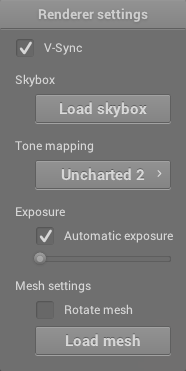
\includegraphics[scale=0.6]{images/renderer_settings.png}
    \end{center}
    %\caption{A megjelenítő beállításai}
\end{wrapfigure}

A megjelenítő beállításai ablakban elsősorban a modelltől független, globális beállítások találhatóak. A V-Sync a vertikális szinkronizáció be- vagy kikapcsolására szolgál. Alapértelmezésben be van kapcsolva, így a megjelenítő mindig megvárja, amíg az elkészült képkocka megjelenítése befejeződik. Ezzel elkerülhető az ún. \textit{tearing}, ha a képernyő frissítési frekvenciájától (jellemzően 60 Hz) eltérő FPS (\textit{frames per second}, képkocka per másodperc) sebességgel dolgozik a megjelenítő. Kikapcsolásával a program az előző képkocka befejezése után egyből elkezdi a következő rajzolását, így ez a mód teljesítménymérésre is alkalmas lehet. 

A \textit{Load skybox} ill. \textit{Load mesh} gombokkal egy fájlválasztó ablak nyílik meg, amelynek segítségével új skybox-ot vagy modellt tölthetünk be. Skybox esetén Radiance HDR (.hdr), modellek esetén Wavefront OBJ (.obj) a támogatott fájlformátum. Továbbá ügyeljünk arra, hogy a skybox-nak megadott kép vertikális kereszt alakban tartalmazza a kockatérkép oldalait.

A \textit{Tone mapping} címke alatt található választógomb segítségével a beépített színleképezési operátorok (Uncharted 2, Reinhard, Unreal 4) közül választhatunk, ill. ki is kapcsolhatjuk a színleképezést az Off bejegyzés választásával.

Az \textit{Exposure} címke alatt lehetőségünk van az automatikus expozíciót be- vagy kikapcsolni. Ez az effektus az emberi szem eltérő fényerősséghez történő alkalmazkodását szimulálja, például amikor egy sötét szobából egy világos térbe lépünk ki. Kikapcsolt állapotában kézzel lehet állítani az expozíciót a lentebb található csúszka segítségével.

Az utolsó beállítás, a \textit{Rotate mesh} jelölőnégyzet segítségével a betöltött modell automatikus forgatását kapcsolhatjuk be/ki.

\subsection{Modell információ}

TODO

\subsection{Anyagtulajdonságok}

\begin{wrapfigure}{l}{0.5\textwidth}
    \begin{center}
        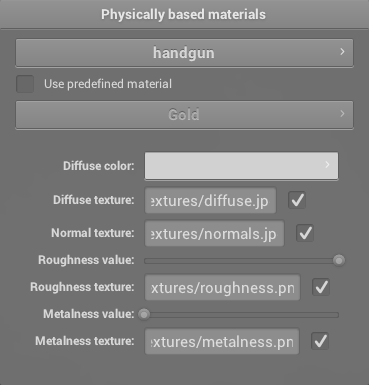
\includegraphics[scale=0.5]{images/pbr_materials.png}
    \end{center}
\end{wrapfigure}

A modellhez tartozó .mtl fájlból olvasott fizikai alapú anyagok a legfelső választógombra kattintva érhetők el, ezek valamelyikére kattintva az ablak tartalma automatikusan frissül.

Amennyiben a modellhez nem volt mellékelve anyagleíró fájl, vagy csak szeretnénk kipróbálni valamilyen valódi anyagot, a \textit{Use predefines material}-t bekapcsolva elérhetővé válik az alatta levő lista, illetve ekkor a modell is a választott előre definiált anyag kinézetével jelenik meg. TODO: anyagok listája ha végleges

Az első anyagtulajdonság a diffúz szín, ami megadható egyetlen színként vagy textúrával is. Ez utóbbi csak akkor elérhető, ha az anyagleíróban volt erre vonatkozó bejegyzés. A hozzátartozó kapcsolóval a beállított szín és (ha elérhető,) a betöltött textúra között válthatunk. A következő tulajdonság a normáltextúra. Ezt is az anyagleíróból olvassa a program, a mellett található jelölőnégyzettel pedig a normáltérképezés kapcsolhatjuk be/ki.

Az utolsó két tulajdonság a fizikai alapú megjelenítéshez tartozik. Az első a rücskösség (\textit{roughness}), amely a felület durvaságát szimbolizálja egy 0 és 1 közé eső értékkel. A tökéletesen sima felületeknél ez az érték 0, míg a legdurvább felületek esetén 1. A diffúz színhez hasonlóan ez az érték is olvasható textúrából, ehhez egy egyedi \textit{map\_Roughness} kulcsot kell az anyagleíró fájlhoz hozzáadnunk. Az utolsó tulajdonság a fémesség (\textit{metalness}), amely a rücskösséghez nagyon hasonlóan működik, csak ennél az adható meg, hogy az anyag szigetelő-e vagy sem. Szigorúan fizikai értelemben ennek értéke csak és kizárólag 0 vagy 1 lehetne, mivel nem tudunk részben szigetelő, részben fémes anyagról. Fontos tudni, hogy ezek az anyagtulajdonságok mindig egy adott felület legkülső rétegét írják le: egy festett fémfelületnél tehát ez az érték 0 lesz, hiszen hiába fém az alapja, a fény a festékről verődik vissza, az pedig fizikailag szigetelő. A fémességet meghatározó textúrát szintén egy egyedi, \textit{map\_Metalness} kulccsal tárolhatjuk el.

\subsection{Megvilágítás beállításai}

TODO